\chapter{Stationary Regression}

\cite{Forster} proposed the last-step min-max prediction rule for online stationary regression.
According to this rule, each round the algorithm assumes that it is the last round,
and outputs the best prediction $\hyi{T}$ assuming the worst choice of the label $\yi{T}$.
Thus, the optimal prediction is\footnote{$\yi{T}$ and $\hyi{T}$ serves both as quantifiers (over the
 $\min$ and $\max$ operators, respectively), and as the optimal values
 over this optimization problem. }
\begin{align}
\hyi{T} = \arg\min_{\hyi{T}} \max_{\yi{T}} \brackets{\sum_{t=1}^{T} (\yi{t} -
  \hyi{t})^2  - \inf_{\vu} \paren{b\left\Vert \mathbf{u}\right\Vert
    ^{2}+L_{T}(\vu)}}~,
\label{forster_minmax}
\end{align}
for some positive constant $b>0$. The first term of \eqref{forster_minmax}
is the loss suffered by the algorithm while the second term is a sum of the loss suffered by a competitor $\mathbf{u}$ and a penalty for the norm of $\mathbf{u}$ to be far from zero.
As we will see, to make the min-max optimization problem well defined,~\cite{Forster} assumed
an artificial bound on the labels $|\yi{t}|\leq Y$, and formally the bound should be known to the learning algorithm.

In \secref{sec:WEMM_alg} we introduce the notation of {\em weighted loss},
where we replace $L_{T}(\vu)$ in \eqref{forster_minmax} with a weighted loss.
This will help us to make the min-max optimization problem well defined (without the need to bound the labels), and
our prediction algorithm will be the formal solution of this problem.
In \secref{sec:WEMM_recursive} we show that our algorithm can be expressed in a recursive form,
similar to other algorithms. In \secref{sec:WEMM_kernel} we show that the algorithm can be expressed in dual variables, which allows an efficient run of the algorithm in any reproducing kernel Hilbert space.
Finally, in \secref{sec:WEMM_comparison} we compare our algorithm to other algorithms of the same form.
The analysis of the algorithm appears in \chapref{chap:WEMM_analysis},
where we derive two regret bounds for the algorithm, and compare them to other bounds.

\section{Weighted Min-Max (WEMM) algorithm}
\label{sec:WEMM_alg}

%Our algorithm is derived based on a last-step min-max prediction,
%proposed by~\cite{Forster}. An algorithm following this approach outputs the
%min-max prediction assuming the current iteration is the last one.
The algorithm we describe below is based on an extension of the last-step min-max rule of~\cite{Forster}.
For this purpose we introduce a weighted cumulative loss using
positive input-dependent weights $\left\{ a_{t}\right\} _{t=1}^{T}$,
\[
L_{T}^{\boldsymbol{a}}(\mathbf{u})=\sum_{t=1}^{T}a_{t}\left(y_{t}-\mathbf{u}^{\top}\mathbf{x}_{t}\right)^{2}
%\quad,\quad
%L_{T}^{\boldsymbol{a}}(\vui{1} \comdots
%\vui{T})=\sum_{t=1}^{T}a_{t}\left(y_{t}-\vuti{t} \vxi{t}\right)^{2}
~.
\]
The exact values of the weights $a_t$ will be defined below.

Our variant of the last-step min-max algorithm predicts
\begin{align}
\hyi{T} = \arg\min_{\hyi{T}} \max_{\yi{T}} \brackets{\sum_{t=1}^{T} (\yi{t} -
  \hyi{t})^2  - \inf_{\vu} \paren{b\left\Vert \mathbf{u}\right\Vert
    ^{2}+L_{T}^{\boldsymbol{a}}(\vu)}}~,
\label{minmax_algorithm_1}
\end{align}
for some positive constant $b>0$.
We next compute the actual prediction based on the optimal last-step min-max solution of \eqref{minmax_algorithm_1}. We
start with additional notation,
\begin{align}
\mathbf{A}_{t}
&=b\mathbf{I}+\sum_{s=1}^{t}a_{s}\mathbf{x}_{s}\mathbf{x}_{s}^{\top}&&\in\mathbb{R}^{d\times
  d}\label{Adef}\\
\mathbf{b}_{t}&=\sum_{s=1}^{t}a_{s}y_{s}\mathbf{x}_{s}&&\in\mathbb{R}^{d}\label{bdef} ~.
\end{align}
The solution of the internal infimum over $\vu$ is summarized in the
following lemma.
\begin{lemma}
\label{lem:lemma1}
For all $t\geq1$, the function $f\left(\mathbf{u}\right)=b\left\Vert \mathbf{u}\right\Vert ^{2}+\sum_{s=1}^{t}a_{s}\left(y_{s}-\mathbf{u}^{\top}\mathbf{x}_{s}\right)^{2}$
is minimal at a unique point $\mathbf{u}_{t}$ given by,
%  Furthermore, $\mathbf{u}_{t}$
% and $f(\mathbf{u}_{t})$ are given by
\begin{align}
\mathbf{u}_{t}=\mathbf{A}_{t}^{-1}\mathbf{b}_{t}\quad\textrm{ and
}\quad
f(\mathbf{u}_{t})=\sum_{s=1}^{t}a_{s}y_{s}^{2}-\mathbf{b}_{t}^{\top}\mathbf{A}_{t}^{-1}\mathbf{b}_{t}
~. \label{optimal_solution}
\end{align}
\end{lemma}
%\kc{please add this proof}
%\edward{Done.}
%The proof is similar to the proof of Lemma 1 by Forster~\cite{Forster}.
\begin{proof}
From
\begin{eqnarray*}
f\left(\mathbf{u}\right) & = & b\left\Vert \mathbf{u}\right\Vert ^{2}+\sum_{s=1}^{t}a_{s}\left(y_{s}-\mathbf{u}^{\top}\mathbf{x}_{s}\right)^{2}\\
 & = & \sum_{s=1}^{t}a_{s}y_{s}^{2}-2\sum_{s=1}^{t}\mathbf{u}^{\top}\left(a_{s}y_{s}\mathbf{x}_{s}\right)+\mathbf{u}^{\top}\left(b\mathbf{I}+\sum_{s=1}^{t}a_{s}\mathbf{x}_{s}\mathbf{x}_{s}^{\top}\right)\mathbf{u}\\
 & \overset{\eqref{Adef},\eqref{bdef}}{=} & \sum_{s=1}^{t}a_{s}y_{s}^{2}-2\mathbf{u}^{\top}\mathbf{b}_{t}+\mathbf{u}^{\top}\mathbf{A}_{t}\mathbf{u}
\end{eqnarray*}
it follows that $\nabla
f\left(\mathbf{u}\right)=2\mathbf{A}_{t}\mathbf{u}-2\mathbf{b}_{t},\:
\triangle f(\mathbf{u})=2\mathbf{A}_{t}\succ 0$.
Thus $f$ is convex and it is minimal if $\nabla f\left(\mathbf{u}\right)=0$,
i.e. for $\mathbf{u}=\mathbf{A}_{t}^{-1}\mathbf{b}_{t}$. This shows
that $\mathbf{u}_{t}=\mathbf{A}_{t}^{-1}\mathbf{b}_{t}$ and we obtain

\[
f\left(\mathbf{u}_{t}\right)=f\left(\mathbf{A}_{t}^{-1}\mathbf{b}_{t}\right)=\sum_{s=1}^{t}a_{s}y_{s}^{2}-2\mathbf{b}_{t}^{\top}\mathbf{A}_{t}^{-1}\mathbf{b}_{t}+\mathbf{b}_{t}^{\top}\mathbf{A}_{t}^{-1}\mathbf{A}_{t}\mathbf{A}_{t}^{-1}\mathbf{b}_{t}=\sum_{s=1}^{t}a_{s}y_{s}^{2}-\mathbf{b}_{t}^{\top}\mathbf{A}_{t}^{-1}\mathbf{b}_{t}~.
\]
\QED
\end{proof}
\begin{Remark}
\label{MAP1}
The minimization problem in \lemref{lem:lemma1} can be interpreted as MAP estimator
of $\mathbf{u}$ based on the sequence $\left\{ \left(\mathbf{x}_{s},y_{s}\right)\right\} _{s=1}^{t}$
in the following generative model:
\begin{eqnarray*}
\mathbf{u} & \sim & N\left(0,\sigma_{b}^{2}\mathbf{I}\right)\\
y_{s} & \sim & N\left(\mathbf{x}_{s}^{\top}\mathbf{u},\sigma_{s}^{2}\right)~,
\end{eqnarray*}
where $\sigma_{b}^{2}=\frac{1}{2b}$ and $\sigma_{s}^{2}=\frac{1}{2a_{s}}$.

Under the model we calculate,
\begin{eqnarray}
\mathbf{u}_{MAP} & = & \arg\max_{\mathbf{u}}P\left(\mathbf{u}\mid\left\{ \mathbf{x}_{s}\right\} ,\left\{ y_{s}\right\} \right) \nonumber \\
 & = & \arg\max_{\mathbf{u}}\left[P\left(\mathbf{u}\right)\prod_{s=1}^{t}P\left(y_{s}\mid\mathbf{u},\mathbf{x}_{s}\right)\right] \nonumber \\
 & = & \arg\min_{\mathbf{u}}\left[-\log P\left(\mathbf{u}\right)-\sum_{s=1}^{t}\log P\left(y_{s}\mid\mathbf{u},\mathbf{x}_{s}\right)\right]~. \label{u_map}
\end{eqnarray}
By our gaussian generative model,
\begin{align*}
&-\log P\left(\mathbf{u}\right)&=&\log\left(2\pi\sigma_{b}^{2}\right)^{d/2}+\frac{1}{2\sigma_{b}^{2}}\left\Vert \mathbf{u}\right\Vert ^{2}\\
&-\log P\left(y_{s}\mid\mathbf{u},\mathbf{x}_{s}\right)&=&\log\left(2\pi\sigma_{s}^{2}\right)^{1/2}+\frac{1}{2\sigma_{s}^{2}}\left(y_{s}-\mathbf{x}_{s}^{\top}\mathbf{u}\right)^{2}~.
\end{align*}
Substituting in \eqref{u_map} we get
\[
 \mathbf{u}_{MAP}=\arg\min_{\mathbf{u}}\left[\frac{1}{2\sigma_{b}^{2}}\left\Vert \mathbf{u}\right\Vert ^{2}+\sum_{s=1}^{t}\frac{1}{2\sigma_{s}^{2}}\left(y_{s}-\mathbf{x}_{s}^{\top}\mathbf{u}\right)^{2}\right]~,
\]
and by using $\frac{1}{2\sigma_{b}^{2}}=b$,
$\frac{1}{2\sigma_{s}^{2}}=a_{s}$ we get the minimization
problem of \lemref{lem:lemma1}.
\end{Remark}

Substituting \eqref{optimal_solution} back in
\eqref{minmax_algorithm_1} we obtain the following form of the min-max
problem,
%
% Before proving the theorem we discuss three possible cases, one
% used by \cite{Forster} and two in the proof of the theorem.
% We show below that one can write the last step minmax problem as
\begin{align}
\min_{\hyi{T}} \max_{\yi{T}} G(\yi{T},\hyi{T}) \quad\textrm{ for }
\quad G(\yi{T},\hyi{T})= \alpha(a_T) \yi{T}^2 + 2 \beta(a_T,
\hyi{T}) \yi{T} + \hyi{T}^2 ~,\label{minmax_objective}
\end{align}
for some functions $\alpha(a_T)$ and $\beta(a_T, \hyi{T})$. Clearly,
for this problem to be well defined the function $G$ should be convex
in $\hyi{T}$ and concave in $\yi{T}$.

A previous choice, proposed by~\cite{Forster}, is to have uniform weights
and set $a_t=1$ (for $t=1 \comdots T$), which for the particular function $\alpha(a_T)$
yields $\alpha(a_T)>0$. Thus, $G(\yi{T},\hyi{T})$ is a convex function
in $\yi{T}$, implying that the optimal value of $G$ is not bounded
from above.~\cite{Forster} addressed this problem by restricting
$\yi{T}$ to belong to a predefined interval $[-Y,Y]$, known also to
the learner. As a consequence, the adversary optimal prediction is in
fact either $\yi{T}=Y$ or $\yi{T}=-Y$, which in turn yields an optimal
predictor which is clipped at this bound, \(
\hat{y}_{T}={\rm clip}\left(\mathbf{b}_{T-1}^{\top}\mathbf{A}_{T}^{-1}\mathbf{x}_{T},Y\right)\),
where for $y>0$ we define ${\rm clip}(x,y)=x$ if $\vert x \vert \leq y$ and
${\rm clip}(x,y) =y\, \sign(x)$, otherwise.
%
\begin{figure}[!t!]
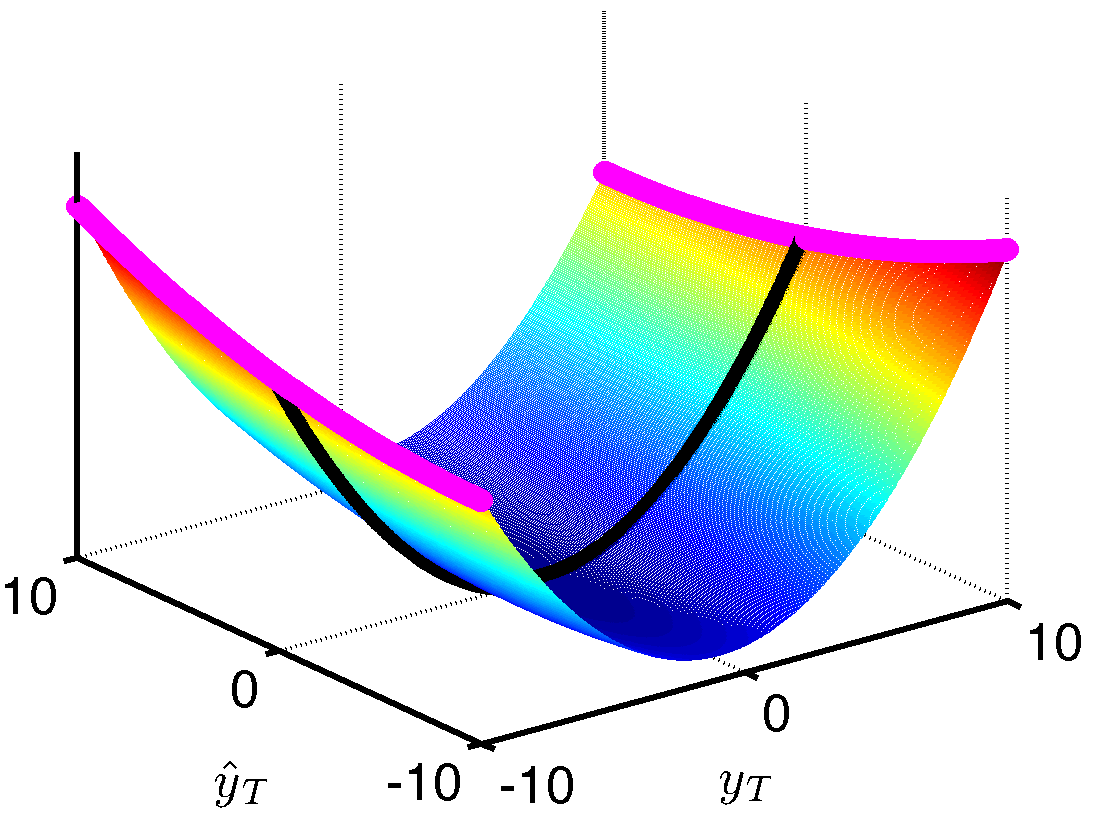
\includegraphics[width=0.32\textwidth]{figs/forster_minmax}
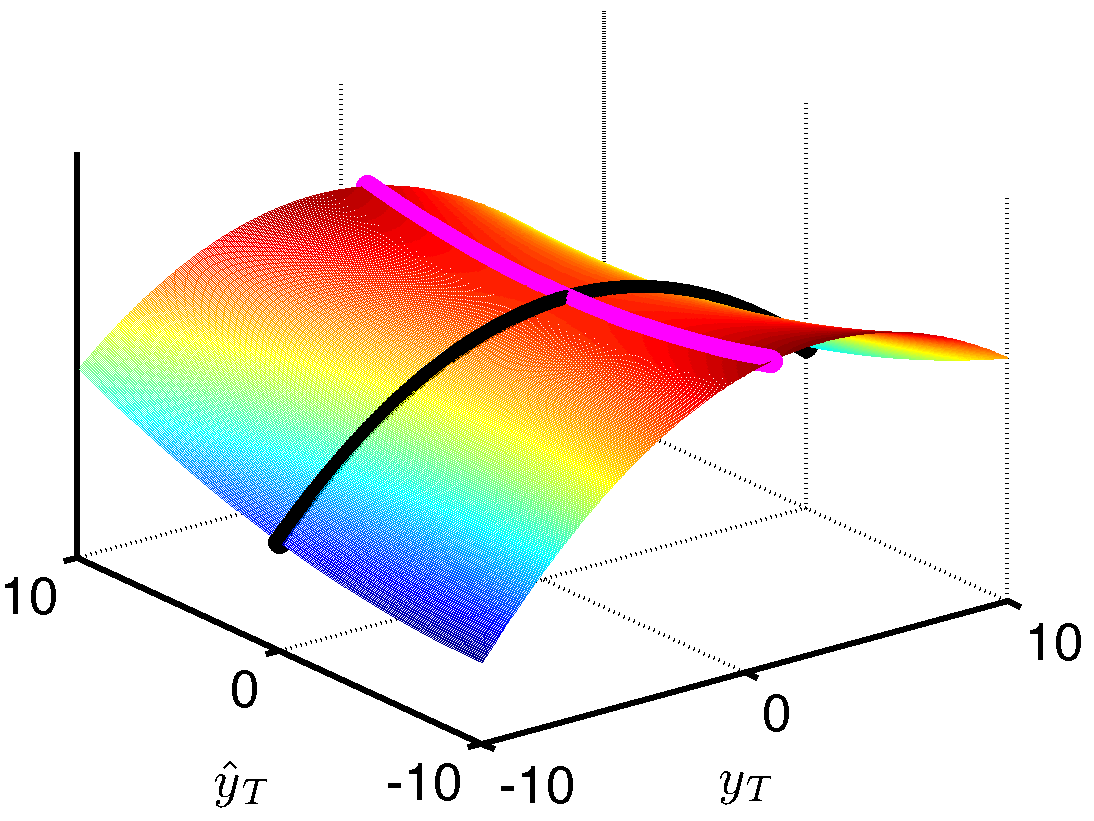
\includegraphics[width=0.32\textwidth]{figs/my_minmax}
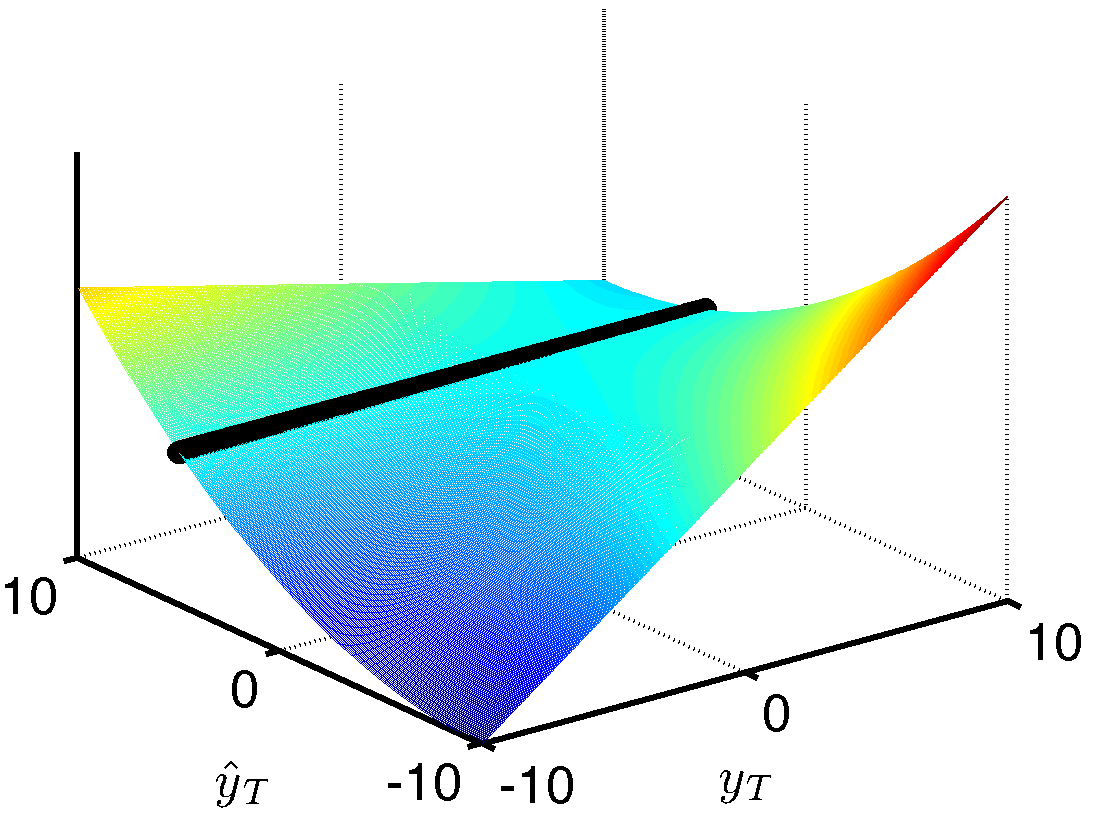
\includegraphics[width=0.32\textwidth]{figs/my_minmax_0}
\caption{
An illustration of the min-max objective function $G(\yi{T},\hyi{T})$
\eqref{minmax_objective}. The black line is the value of the objective
as a function of $\yi{T}$ for the optimal predictor $\hyi{T}$.
Left: Forster's optimization function (convex in $\yi{T}$).
Center: our optimization function (strictly  concave in $\yi{T}$,
case 1 in \thmref{thm:theorem1}).
Right: our optimization function (invariant to $\yi{T}$, case 2 in \thmref{thm:theorem1}).}
\label{fig:minmax}
\end{figure}
%

This phenomena is illustrated in the left panel
of \figref{fig:minmax} (best viewed in color).  For the min-max optimization function defined
by~\cite{Forster}, fixing some value of $\hat{y}_{T}$, the function
is convex in $y_{T}$, and the adversary would achieve a maximal value
at the boundary of the feasible values of $y_{T}$ interval. That is,
either $y_{T}=Y$ or $y_{T}=-Y$, as indicated by the two magenta lines
at $\yi{T}=\pm10$. The optimal predictor $\hat{y}_{T}$ is
achieved somewhere along the lines $y_{T}=Y$ or $y_{T}=-Y$.

% and showed that it is optimal when the last outcome variable is bounded,
% that is $y_{T}\in[-Y,Y]$. We next give similar result, but we do
% not assume that $y_{T}$ is bounded. Instead, other assumption is
% required.

% The difference between our and Forster optimization function is illustrated
% in the next figure:

We propose an alternative approach to make the min-max optimal solution
bounded by appropriately setting the weight $a_T$ such that
$G(\yi{T},\hyi{T})$ is concave in $\yi{T}$ for a constant
$\hat{y}_{T}$. We explicitly consider two cases.
%
First, set $a_T$ such that $G(\yi{T},\hyi{T})$ is {\em strictly
  concave} in $\yi{T}$, and thus attains a single maximum with no need
to artificially restrict the value of $\yi{T}$. The optimal predictor
$\hat{y}_{T}$ in this case is achieved in the unique saddle point, as illustrated
in the center panel of \figref{fig:minmax}.
%
A second case is to set $a_T$ such that $\alpha(a_T)=0$ and the
min-max function $G(\yi{T},\hyi{T})$ becomes linear in $\yi{T}$. Here,
the optimal prediction is achieved by choosing $\hyi{T}$ such that
$\beta(a_T, \hyi{T})=0$ which turns $G(\yi{T},\hyi{T})$ to be
invariant to $\yi{T}$, as illustrated in the right panel of
\figref{fig:minmax}.  % the for a
% specific choice of $\hat{y}_{T}$, because for other $\hat{y}_{T}$ the
% optimization function can made large by choosing $y_{T}$ with large
% absolute value.

Equipped with
\lemref{lem:lemma1} we develop the optimal solution of the min-max
predictor, summarized in the following theorem.
%
\begin{theorem}
\label{thm:theorem1}
Assume that $1+a_{T}\mathbf{x}_{T}^{\top}\mathbf{A}_{T-1}^{-1}\mathbf{x}_{T}-a_{T}\leq0$.
Then the optimal prediction for the last round $T$ is
\begin{align}
\hat{y}_{T}=\mathbf{b}_{T-1}^{\top}\mathbf{A}_{T-1}^{-1}\mathbf{x}_{T}
~. \label{laststep_minmax_optimal}
\end{align}
\end{theorem}
%
%The proof appears in \secref{proof_theorem1}
The proof of the theorem makes use of the following technical lemma.
\begin{lemma}
\label{lem:lemma2}
For all $t=1,2,\ldots,T$
\begin{equation}
a_{t}^{2}\mathbf{x}_{t}^{\top}\mathbf{A}_{t}^{-1}\mathbf{x}_{t}+1-a_{t}=\frac{1+a_{t}\mathbf{x}_{t}^{\top}\mathbf{A}_{t-1}^{-1}\mathbf{x}_{t}-a_{t}}{1+a_{t}\mathbf{x}_{t}^{\top}\mathbf{A}_{t-1}^{-1}\mathbf{x}_{t}}
~. \label{lemma2}
\end{equation}
\end{lemma}
\begin{proof}
Using the Woodbury identity we get
\[
\mathbf{A}_{t}^{-1}=\mathbf{A}_{t-1}^{-1}-\frac{\mathbf{A}_{t-1}^{-1}\mathbf{x}_{t}\mathbf{x}_{t}^{\top}\mathbf{A}_{t-1}^{-1}}{\frac{1}{a_{t}}+\mathbf{x}_{t}^{\top}\mathbf{A}_{t-1}^{-1}\mathbf{x}_{t}}~,
\]
 therefore the left side of \eqref{lemma2} is
\begin{eqnarray*}
a_{t}^{2}\mathbf{x}_{t}^{\top}\mathbf{A}_{t}^{-1}\mathbf{x}_{t}+1-a_{t}
 &=&  a_{t}^{2}\mathbf{x}_{t}^{\top}\left(\mathbf{A}_{t-1}^{-1}-\frac{\mathbf{A}_{t-1}^{-1}\mathbf{x}_{t}\mathbf{x}_{t}^{\top}\mathbf{A}_{t-1}^{-1}}{\frac{1}{a_{t}}+\mathbf{x}_{t}^{\top}\mathbf{A}_{t-1}^{-1}\mathbf{x}_{t}}\right)\mathbf{x}_{t}+1-a_{t}\\
  &=&  a_{t}^{2}\mathbf{x}_{t}^{\top}\mathbf{A}_{t-1}^{-1}\mathbf{x}_{t}-\frac{a_{t}^{2}\mathbf{x}_{t}^{\top}\mathbf{A}_{t-1}^{-1}\mathbf{x}_{t}\mathbf{x}_{t}^{\top}\mathbf{A}_{t-1}^{-1}\mathbf{x}_{t}}{\frac{1}{a_{t}}+\mathbf{x}_{t}^{\top}\mathbf{A}_{t-1}^{-1}\mathbf{x}_{t}}+1-a_{t}\\
  &=&  \frac{1+a_{t}\mathbf{x}_{t}^{\top}\mathbf{A}_{t-1}^{-1}\mathbf{x}_{t}-a_{t}}{1+a_{t}\mathbf{x}_{t}^{\top}\mathbf{A}_{t-1}^{-1}\mathbf{x}_{t}}~.
\end{eqnarray*}
\QED
 \end{proof}
We now prove \thmref{thm:theorem1}.
\begin{proof}
The adversary can choose any $y_{T}$, thus the algorithm should predict
$\hat{y}_{T}$ such that the following quantity is minimal,
\begin{eqnarray*}
&&\max_{y_{T}}\left(\sum_{t=1}^{T}\left(y_{t}-\hat{y}_{t}\right)^{2}-\inf_{\mathbf{u}\in\mathbb{R}^{d}}\left(b\left\Vert \mathbf{u}\right\Vert ^{2}+\sum_{t=1}^{T}a_{t}\left(y_{t}-\mathbf{u}^{\top}\mathbf{x}_{t}\right)^{2}\right)\right)\\
&\overset{\eqref{optimal_solution}}{=}&\max_{y_{T}}\left(\sum_{t=1}^{T}\left(y_{t}-\hat{y}_{t}\right)^{2}-\sum_{t=1}^{T}a_{t}y_{t}^{2}+\mathbf{b}_{T}^{\top}\mathbf{A}_{T}^{-1}\mathbf{b}_{T}\right) ~.
\end{eqnarray*}
That is, we need to solve the following min-max problem
\[
\min_{\hat{y}_{T}}\max_{y_{T}}\left(\sum_{t=1}^{T}\left(y_{t}-\hat{y}_{t}\right)^{2}-\sum_{t=1}^{T}a_{t}y_{t}^{2}+\mathbf{b}_{T}^{\top}\mathbf{A}_{T}^{-1}\mathbf{b}_{T}\right)~.
\]
We use the following relation to re-write the optimization problem,
\begin{align}
\mathbf{b}_{T}^{\top}\mathbf{A}_{T}^{-1}\mathbf{b}_{T}
%& = & \left(\mathbf{b}_{T-1}+a_{T}y_{T}\mathbf{x}_{T}\right)^{\top}\mathbf{A}_{T}^{-1}\left(\mathbf{b}_{T-1}+a_{T}y_{T}\mathbf{x}_{T}\right)\nonumber \\
 & = &
 \mathbf{b}_{T-1}^{\top}\mathbf{A}_{T}^{-1}\mathbf{b}_{T-1}+2a_{T}y_{T}\mathbf{b}_{T-1}^{\top}\mathbf{A}_{T}^{-1}\mathbf{x}_{T}+a_{T}^{2}y_{T}^{2}\mathbf{x}_{T}^{\top}\mathbf{A}_{T}^{-1}\mathbf{x}_{T} ~.\label{t3}
\end{align}
Omitting all terms that are
not depending on $y_{T}$ and $\hat{y}_{T}$,
\[
\min_{\hat{y}_{T}}\max_{y_{T}}\left(\left(y_{T}-\hat{y}_{T}\right)^{2}-a_{T}y_{T}^{2}+2a_{T}y_{T}\mathbf{b}_{T-1}^{\top}\mathbf{A}_{T}^{-1}\mathbf{x}_{T}+a_{T}^{2}y_{T}^{2}\mathbf{x}_{T}^{\top}\mathbf{A}_{T}^{-1}\mathbf{x}_{T}\right)~.
\]
We manipulate the last problem to be of form \eqref{minmax_objective} using \lemref{lem:lemma2},
% \[
% \min_{\hat{y}_{T}}\max_{y_{T}}\left(\left(a_{T}^{2}\mathbf{x}_{T}^{\top}\mathbf{A}_{T}^{-1}\mathbf{x}_{T}+1-a_{T}\right)y_{T}^{2}+2y_{T}\left(a_{T}\mathbf{b}_{T-1}^{\top}\mathbf{A}_{T}^{-1}\mathbf{x}_{T}-\hat{y}_{T}\right)+\hat{y}_{T}^{2}\right)
% \]
% and by lemma 2 we get
\begin{align}
\min_{\hat{y}_{T}}\max_{y_{T}} \left(\!
  \frac{1+a_{T}\mathbf{x}_{T}^{\top}\mathbf{A}_{T-1}^{-1}\mathbf{x}_{T}-a_{T}}{1+a_{T}\mathbf{x}_{T}^{\top}\mathbf{A}_{T-1}^{-1}\mathbf{x}_{T}}y_{T}^{2}+2y_{T}\left(a_{T}\mathbf{b}_{T-1}^{\top}\mathbf{A}_{T}^{-1}\mathbf{x}_{T}-\hat{y}_{T}\right)+\hat{y}_{T}^{2}
\!\right),\label{minmax}
\end{align}
where
\[
\alpha(a_T)=\frac{1+a_{T}\mathbf{x}_{T}^{\top}\mathbf{A}_{T-1}^{-1}\mathbf{x}_{T}-a_{T}}{1+a_{T}\mathbf{x}_{T}^{\top}\mathbf{A}_{T-1}^{-1}\mathbf{x}_{T}}
\quad\textrm{ and }\quad
\beta(a_T,\hyi{T})=a_{T}\mathbf{b}_{T-1}^{\top}\mathbf{A}_{T}^{-1}\mathbf{x}_{T}-\hat{y}_{T}~.
\]

We consider two cases:  (1)
$1+a_{T}\mathbf{x}_{T}^{\top}\mathbf{A}_{T-1}^{-1}\mathbf{x}_{T}-a_{T}<0$
(corresponding to the middle panel of \figref{fig:minmax}),
and (2)
$1+a_{T}\mathbf{x}_{T}^{\top}\mathbf{A}_{T-1}^{-1}\mathbf{x}_{T}-a_{T}=0$
(corresponding to the right panel of \figref{fig:minmax}),
starting with the first case,
\begin{equation}
1+a_{T}\mathbf{x}_{T}^{\top}\mathbf{A}_{T-1}^{-1}\mathbf{x}_{T}-a_{T}<0\label{option1}~.
\end{equation}
Denote the inner-maximization problem by,
\[
f\left(y_{T}\right)\!=\!\frac{1+a_{T}\mathbf{x}_{T}^{\top}\mathbf{A}_{T-1}^{-1}\mathbf{x}_{T}-a_{T}}{1+a_{T}\mathbf{x}_{T}^{\top}\mathbf{A}_{T-1}^{-1}\mathbf{x}_{T}}y_{T}^{2}+2y_{T}\left(a_{T}\mathbf{b}_{T-1}^{\top}\mathbf{A}_{T}^{-1}\mathbf{x}_{T}-\hat{y}_{T}\right)+\hat{y}_{T}^{2}~. 
\]
This function is strictly-concave with respect to $y_{T}$ because of
\eqref{option1}. Thus, it has a unique maximal value given by,
\begin{eqnarray*}
f^{max}(\hyi{T})
%& = & \hat{y}_{T}^{2}-\frac{\left(a_{T}\mathbf{b}_{T-1}^{\top}\mathbf{A}_{T}^{-1}\mathbf{x}_{T}-\hat{y}_{T}\right)^{2}\left(1+a_{T}\mathbf{x}_{T}^{\top}\mathbf{A}_{T-1}^{-1}\mathbf{x}_{T}\right)}{1+a_{T}\mathbf{x}_{T}^{\top}\mathbf{A}_{T-1}^{-1}\mathbf{x}_{T}-a_{T}}\\
 & = & -\frac{a_{T}}{1+a_{T}\mathbf{x}_{T}^{\top}\mathbf{A}_{T-1}^{-1}\mathbf{x}_{T}-a_{T}}\hat{y}_{T}^{2}+\frac{2a_{T}\mathbf{b}_{T-1}^{\top}\mathbf{A}_{T}^{-1}\mathbf{x}_{T}\left(1+a_{T}\mathbf{x}_{T}^{\top}\mathbf{A}_{T-1}^{-1}\mathbf{x}_{T}\right)}{1+a_{T}\mathbf{x}_{T}^{\top}\mathbf{A}_{T-1}^{-1}\mathbf{x}_{T}-a_{T}}\hat{y}_{T}\\
 &  & -\frac{\left(a_{T}\mathbf{b}_{T-1}^{\top}\mathbf{A}_{T}^{-1}\mathbf{x}_{T}\right)^{2}\left(1+a_{T}\mathbf{x}_{T}^{\top}\mathbf{A}_{T-1}^{-1}\mathbf{x}_{T}\right)}{1+a_{T}\mathbf{x}_{T}^{\top}\mathbf{A}_{T-1}^{-1}\mathbf{x}_{T}-a_{T}}~.
\end{eqnarray*}
Next, we solve $\min_{\hat{y}_{T}} f^{max}( \hyi{T} )$, which is strictly-convex
with respect to $\hat{y}_{T}$ because of \eqref{option1}. Solving this problem we get the optimal
last-step min-max predictor,
\begin{equation}
\hat{y}_{T}=\mathbf{b}_{T-1}^{\top}\mathbf{A}_{T}^{-1}\mathbf{x}_{T}\left(1+a_{T}\mathbf{x}_{T}^{\top}\mathbf{A}_{T-1}^{-1}\mathbf{x}_{T}\right)
~.
\label{t1}
\end{equation}
We further derive the last equation. From \eqref{Adef} we have,
\begin{equation}
\mathbf{A}_{T}^{-1}a_{T}\mathbf{x}_{T}\mathbf{x}_{T}^{\top}\mathbf{A}_{T-1}^{-1}=\mathbf{A}_{T}^{-1}\left(\mathbf{A}_{T}-\mathbf{A}_{T-1}\right)\mathbf{A}_{T-1}^{-1}=\mathbf{A}_{T-1}^{-1}-\mathbf{A}_{T}^{-1}\label{t2}~.
\end{equation}
Substituting \eqref{t2} in \eqref{t1} we have the following equality
as desired,
\begin{align}
\hat{y}_{T} & =  \mathbf{b}_{T-1}^{\top}\mathbf{A}_{T}^{-1}\mathbf{x}_{T}+\mathbf{b}_{T-1}^{\top}\mathbf{A}_{T}^{-1}a_{T}\mathbf{x}_{T}\mathbf{x}_{T}^{\top}\mathbf{A}_{T-1}^{-1}\mathbf{x}_{T}
 %& =  \mathbf{b}_{T-1}^{\top}\mathbf{A}_{T}^{-1}\mathbf{x}_{T}+\mathbf{b}_{T-1}^{\top}\left(\mathbf{A}_{T-1}^{-1}-\mathbf{A}_{T}^{-1}\right)\mathbf{x}_{T}\\
  =  \mathbf{b}_{T-1}^{\top}\mathbf{A}_{T-1}^{-1}\mathbf{x}_{T}~. \label{t3_thm}
\end{align}
%as desired.

We now move to the second case for which,
\(
1+a_{T}\mathbf{x}_{T}^{\top}\mathbf{A}_{T-1}^{-1}\mathbf{x}_{T}-a_{T}=0,
\)
which is written equivalently as,
\begin{equation}
a_{T}=\frac{1}{1-\mathbf{x}_{T}^{\top}\mathbf{A}_{T-1}^{-1}\mathbf{x}_{T}}
~. \label{aT}
\end{equation}
Substituting \eqref{aT} in \eqref{minmax} we get,
\[
\min_{\hat{y}_{T}}\max_{y_{T}}\left(2y_{T}\left(a_{T}\mathbf{b}_{T-1}^{\top}\mathbf{A}_{T}^{-1}\mathbf{x}_{T}-\hat{y}_{T}\right)+\hat{y}_{T}^{2}\right) ~.
\]
For $\hat{y}_{T}\neq
a_{T}\mathbf{b}_{T-1}^{\top}\mathbf{A}_{T}^{-1}\mathbf{x}_{T}$, the
value of the optimization problem is not-bounded as the adversary
may choose $\yi{T} =z^2
\left(a_{T}\mathbf{b}_{T-1}^{\top}\mathbf{A}_{T}^{-1}\mathbf{x}_{T}-\hat{y}_{T}\right)
$ for $z\rightarrow\infty$. Thus, the optimal last-step min-max prediction
is to set
$\hat{y}_{T}=a_{T}\mathbf{b}_{T-1}^{\top}\mathbf{A}_{T}^{-1}\mathbf{x}_{T}$.
Substituting $a_T =
1+a_{T}\mathbf{x}_{T}^{\top}\mathbf{A}_{T-1}^{-1}\mathbf{x}_{T}$ and
following the derivation from \eqref{t1} to \eqref{t3_thm} above, yields the
desired identity.
%
% To show that it is equal to
% $\mathbf{b}_{T-1}^{\top}\mathbf{A}_{T-1}^{-1}\mathbf{x}_{T}$ we use
% the Woodbury identity and get
% \begin{eqnarray*}
% \mathbf{A}_{T}^{-1} & = & \mathbf{A}_{T-1}^{-1}-\frac{\mathbf{A}_{T-1}^{-1}\mathbf{x}_{T}\mathbf{x}_{T}^{\top}\mathbf{A}_{T-1}^{-1}}{\frac{1}{a_{T}}+\mathbf{x}_{T}^{\top}\mathbf{A}_{T-1}^{-1}\mathbf{x}_{T}}\\
%  & \overset{\eqref{aT}}{=} & \mathbf{A}_{T-1}^{-1}-\frac{\mathbf{A}_{T-1}^{-1}\mathbf{x}_{T}\mathbf{x}_{T}^{\top}\mathbf{A}_{T-1}^{-1}}{1-\mathbf{x}_{T}^{\top}\mathbf{A}_{T-1}^{-1}\mathbf{x}_{T}+\mathbf{x}_{T}^{\top}\mathbf{A}_{T-1}^{-1}\mathbf{x}_{T}}\\
%  & = & \mathbf{A}_{T-1}^{-1}-\mathbf{A}_{T-1}^{-1}\mathbf{x}_{T}\mathbf{x}_{T}^{\top}\mathbf{A}_{T-1}^{-1}
% \end{eqnarray*}
%  therefore $\hat{y}_{T}$ can be written as
% \begin{eqnarray*}
% \hat{y}_{T} & = & a_{T}\mathbf{b}_{T-1}^{\top}\left(\mathbf{A}_{T-1}^{-1}-\mathbf{A}_{T-1}^{-1}\mathbf{x}_{T}\mathbf{x}_{T}^{\top}\mathbf{A}_{T-1}^{-1}\right)\mathbf{x}_{T}\\
%  & \overset{\eqref{aT}}{=} & \frac{1}{1-\mathbf{x}_{T}^{\top}\mathbf{A}_{T-1}^{-1}\mathbf{x}_{T}}\mathbf{b}_{T-1}^{\top}\mathbf{A}_{T-1}^{-1}\mathbf{x}_{T}\left(1-\mathbf{x}_{T}^{\top}\mathbf{A}_{T-1}^{-1}\mathbf{x}_{T}\right)\\
%  & = & \mathbf{b}_{T-1}^{\top}\mathbf{A}_{T-1}^{-1}\mathbf{x}_{T}
% \end{eqnarray*}
 \QED\end{proof}
% \begin{proof}
% Using the Woodbury matrix identity we get
% \begin{eqnarray}
% \mathbf{A}_{t}^{-1} & = & \mathbf{A}_{t-1}^{-1}-\frac{\mathbf{A}_{t-1}^{-1}\mathbf{x}_{t}\mathbf{x}_{t}^{\top}\mathbf{A}_{t-1}^{-1}}{\frac{1}{a_{t}}+\mathbf{x}_{t}^{\top}\mathbf{A}_{t-1}^{-1}\mathbf{x}_{t}}\label{woodbury}
% \end{eqnarray}
% therefore
% \begin{eqnarray}
% \mathbf{A}_{t}^{-1}\mathbf{x}_{t} & = & \mathbf{A}_{t-1}^{-1}\mathbf{x}_{t}-\frac{\mathbf{A}_{t-1}^{-1}\mathbf{x}_{t}\mathbf{x}_{t}^{\top}\mathbf{A}_{t-1}^{-1}\mathbf{x}_{t}}{\frac{1}{a_{t}}+\mathbf{x}_{t}^{\top}\mathbf{A}_{t-1}^{-1}\mathbf{x}_{t}}\nonumber \\
%  & = & \frac{\mathbf{A}_{t-1}^{-1}\mathbf{x}_{t}}{1+a_{t}\mathbf{x}_{t}^{\top}\mathbf{A}_{t-1}^{-1}\mathbf{x}_{t}}\label{t4}
% \end{eqnarray}
% For $1\leq t\leq T$ we have
% \begin{eqnarray*}
%  &  & \ell_{t}(\textrm{alg})+\min_{\mathbf{u}\in\mathbb{R}^{d}}\left(b\left\Vert \mathbf{u}\right\Vert ^{2}+L_{t-1}^{\boldsymbol{a}}(\mathbf{u})\right)-\min_{\mathbf{u}\in\mathbb{R}^{d}}\left(b\left\Vert \mathbf{u}\right\Vert ^{2}+L_{t}^{\boldsymbol{a}}(\mathbf{u})\right)\\
%  &  & =\left(y_{t}-\hat{y}_{t}\right)^{2}+\min_{\mathbf{u}\in\mathbb{R}^{d}}\left(b\left\Vert \mathbf{u}\right\Vert ^{2}+\sum_{s=1}^{t-1}a_{s}\left(y_{s}-\mathbf{u}^{\top}\mathbf{x}_{s}\right)^{2}\right)-\min_{\mathbf{u}\in\mathbb{R}^{d}}\left(b\left\Vert \mathbf{u}\right\Vert ^{2}+\sum_{s=1}^{t}a_{s}\left(y_{s}-\mathbf{u}^{\top}\mathbf{x}_{s}\right)^{2}\right)\\
%  &  & \overset{Lemma1}{=}\left(y_{t}-\hat{y}_{t}\right)^{2}+\sum_{s=1}^{t-1}a_{s}y_{s}^{2}-\mathbf{b}_{t-1}^{\top}\mathbf{A}_{t-1}^{-1}\mathbf{b}_{t-1}-\sum_{s=1}^{t}a_{s}y_{s}^{2}+\mathbf{b}_{t}^{\top}\mathbf{A}_{t}^{-1}\mathbf{b}_{t}\\
%  &  & =\left(y_{t}-\hat{y}_{t}\right)^{2}-a_{t}y_{t}^{2}-\mathbf{b}_{t-1}^{\top}\mathbf{A}_{t-1}^{-1}\mathbf{b}_{t-1}+\mathbf{b}_{t}^{\top}\mathbf{A}_{t}^{-1}\mathbf{b}_{t}\\
%  &  & \overset{\eqref{t3}}{=}\left(y_{t}-\hat{y}_{t}\right)^{2}-a_{t}y_{t}^{2}-\mathbf{b}_{t-1}^{\top}\mathbf{A}_{t-1}^{-1}\mathbf{b}_{t-1}+\mathbf{b}_{t-1}^{\top}\mathbf{A}_{t}^{-1}\mathbf{b}_{t-1}+2a_{t}y_{t}\mathbf{b}_{t-1}^{\top}\mathbf{A}_{t}^{-1}\mathbf{x}_{t}+a_{t}^{2}y_{t}^{2}\mathbf{x}_{t}^{\top}\mathbf{A}_{t}^{-1}\mathbf{x}_{t}\\
%  &  & =\left(y_{t}-\hat{y}_{t}\right)^{2}-a_{t}y_{t}^{2}-\mathbf{b}_{t-1}^{\top}\left(\mathbf{A}_{t-1}^{-1}-\mathbf{A}_{t}^{-1}\right)\mathbf{b}_{t-1}+2a_{t}y_{t}\mathbf{b}_{t-1}^{\top}\mathbf{A}_{t}^{-1}\mathbf{x}_{t}+a_{t}^{2}y_{t}^{2}\mathbf{x}_{t}^{\top}\mathbf{A}_{t}^{-1}\mathbf{x}_{t}\\
%  &  & \overset{\eqref{t2}}{=}\left(y_{t}-\hat{y}_{t}\right)^{2}-a_{t}y_{t}^{2}-\mathbf{b}_{t-1}^{\top}\mathbf{A}_{t}^{-1}a_{t}\mathbf{x}_{t}\mathbf{x}_{t}^{\top}\mathbf{A}_{t-1}^{-1}\mathbf{b}_{t-1}+2a_{t}y_{t}\mathbf{b}_{t-1}^{\top}\mathbf{A}_{t}^{-1}\mathbf{x}_{t}+a_{t}^{2}y_{t}^{2}\mathbf{x}_{t}^{\top}\mathbf{A}_{t}^{-1}\mathbf{x}_{t}\\
%  &  & =\left(y_{t}-\hat{y}_{t}\right)^{2}-a_{t}y_{t}^{2}+a_{t}\left(-\hat{y}_{t}\mathbf{b}_{t-1}^{\top}+2y_{t}\mathbf{b}_{t-1}^{\top}+a_{t}y_{t}^{2}\mathbf{x}_{t}^{\top}\right)\mathbf{A}_{t}^{-1}\mathbf{x}_{t}\\
%  &  & \overset{\eqref{t4}}{=}\left(y_{t}-\hat{y}_{t}\right)^{2}-a_{t}y_{t}^{2}+a_{t}\left(-\hat{y}_{t}\mathbf{b}_{t-1}^{\top}+2y_{t}\mathbf{b}_{t-1}^{\top}+a_{t}y_{t}^{2}\mathbf{x}_{t}^{\top}\right)\frac{\mathbf{A}_{t-1}^{-1}\mathbf{x}_{t}}{1+a_{t}\mathbf{x}_{t}^{\top}\mathbf{A}_{t-1}^{-1}\mathbf{x}_{t}}\\
%  &  & =\left(y_{t}-\hat{y}_{t}\right)^{2}+a_{t}\frac{-y_{t}^{2}-y_{t}^{2}a_{t}\mathbf{x}_{t}^{\top}\mathbf{A}_{t-1}^{-1}\mathbf{x}_{t}-\hat{y}_{t}^{2}+2y_{t}\hat{y}_{t}+a_{t}y_{t}^{2}\mathbf{x}_{t}^{\top}\mathbf{A}_{t-1}^{-1}\mathbf{x}_{t}}{1+a_{t}\mathbf{x}_{t}^{\top}\mathbf{A}_{t-1}^{-1}\mathbf{x}_{t}}\\
%  &  & =\left(y_{t}-\hat{y}_{t}\right)^{2}-a_{t}\frac{\left(y_{t}-\hat{y}_{t}\right)^{2}}{1+a_{t}\mathbf{x}_{t}^{\top}\mathbf{A}_{t-1}^{-1}\mathbf{x}_{t}}\\
%  &  & =\frac{1+a_{t}\mathbf{x}_{t}^{\top}\mathbf{A}_{t-1}^{-1}\mathbf{x}_{t}-a_{t}}{1+a_{t}\mathbf{x}_{t}^{\top}\mathbf{A}_{t-1}^{-1}\mathbf{x}_{t}}\left(y_{t}-\hat{y}_{t}\right)^{2}\leq0
% \end{eqnarray*}
% Summing over $t\in\left\{ 1,\ldots,T\right\} $ we get, %and using \eqref{LT}
% gives
% \[
% L_{T}(\textrm{alg})-\min_{\mathbf{u}\in\mathbb{R}^{d}}\left(b\left\Vert \mathbf{u}\right\Vert ^{2}+L_{T}^{\boldsymbol{a}}(\mathbf{u})\right)\leq0
% \]
 %
% \QED\end{proof}
 %
% \subsection{consume here}
%
% Our algorithm
%
% For our first algorithm we propose a variant of this algorithm which
% solves the following prpblem
%
% In\cite{Forster}, Forster proposed the following predictor for the last
% round
% \[
% \hat{y}_{T}=clip\left(\mathbf{b}_{T-1}^{\top}\mathbf{A}_{T}^{-1}\mathbf{x}_{T},Y\right)
% \]
% and showed that it is optimal when the last outcome variable is bounded,
% that is $y_{T}\in[-Y,Y]$. We next give similar result, but we do
% not assume that $y_{T}$ is bounded. Instead, other assumption is
% required.
%
% \cite{Forster} solved a variant of this problem, yet because the
% problem is convex in $\yi{T}$ kkk
%
% predicts a
% $\paren{\vxti{t}\vwi{t-1}-\yi{t}}^2$
% We will show below that a
% min-max algorithm also chooses a linear function, that is we have,
% $\hyi{t} = \vxti{t}\vwi{t-1}$ for some $\vwi{t-1}\in\reals^d$.

% We will also use an extended notion of evaluation, comparing
% our algorithm to a sequence of functions,
%
%  where there is some restriction over the sequence
%  ${\vui{1}\comdots\vui{T}}$.
%
% This generalization will help us to get results for more complex scenarios,
% such as non-stationary models.
%
%
% In this section we calculate the best prediction for Learner in the
% last round and we prove an upper bound on the regret for linear regression
% with square loss. Unlike\cite{Forster}, we do not assume here that the outcome
% variable is bounded.
%
% Like in\cite{Forster}, we consider the following protocol of interaction
% between Learner and adversary: \\
% FOR $t=1,2,3,\ldots,T$
% \begin{itemize}
% \item adversary chooses an instance $\mathbf{x}_{t}\in\mathbb{R}^{d}$
% \item learner chooses a prediction $\hat{y}_{t}\in\mathbb{R}$
% \item adversary chooses an outcome $y_{t}\in\mathbb{R}$
% \end{itemize}
% END FOR
%
% \noindent \begin{flushleft}
% At each round $t$ the loss of the learner is
% \par\end{flushleft}
%
% \noindent \begin{flushleft}
% \[
% \ell_{t}(\textrm{alg})=\left(y_{t}-\hat{y}_{t}\right)^{2}
% \]
% and after $T$ rounds, the total loss of the learner is
% \par\end{flushleft}
%
% \begin{equation}
% L_{T}(\textrm{alg})=\sum_{t=1}^{T}\ell_{t}(\textrm{alg})\label{LT}
% \end{equation}
%

We conclude by noting that although we did not restrict the form of
the predictor $\hyi{T}$, it turns out that it is a linear predictor
defined by $\hyi{T} = \vxti{T}\vwi{T-1}$ for $\vwi{T-1} =
\mathbf{A}_{T-1}^{-1}\mathbf{b}_{T-1}$. In other words, the functional
form of the optimal predictor is the same as the form of the
comparison function class - linear functions in our case. We call the
algorithm (defined using \eqref{Adef}, \eqref{bdef} and
\eqref{laststep_minmax_optimal}) \texttt{WEMM} for weighted min-max
prediction, and it is summarised in \figref{algorithm:WEMM}.
We note that \texttt{WEMM}
can also be seen as an incremental off-line
algorithm~\citep{AzouryWa01} or follow-the-leader, on a
weighted sequence: The prediction $\hyi{T} =
\vxti{T}\vwi{T-1}$ is with a model that is optimal over a prefix of length $T-1$.  The prediction of the optimal
predictor defined in \eqref{optimal_solution} is
$\vxti{T}\mathbf{u}_{T-1}=\vxti{T}\mathbf{A}_{T-1}^{-1}\mathbf{b}_{T-1}=\hat{y}_T$,
where $\hat{y}_T$ was defined in \eqref{laststep_minmax_optimal}.

\begin{figure}[t]
{
\paragraph{Parameter:} $1<b$
\paragraph{Initialize:} Set
$\mathbf{A}_{0}=b\,\mathbf{I}\in\reals^{d\times d}$ and
$\mathbf{b}_0=\vzero\in\reals^d$\\
{\bf For $t=1 \comdots T$} do
\begin{itemize}
\nolineskips
\item Receive an instance $\vxi{t}$
\item Output  prediction $\hyi{t}=\mathbf{b}_{t-1}^{\top}\mathbf{A}_{t-1}^{-1}\mathbf{x}_{t}$
\item Receive the correct label $\yi{t}$
\item
Set weight:
\begin{align*}
a_{t}&=\frac{1}{1-\mathbf{x}_{t}^{\top}\mathbf{A}_{t-1}^{-1}\mathbf{x}_{t}}
\end{align*}
\item
Update:
\begin{align*}
\mathbf{A}_{t}&=\mathbf{A}_{t-1}+a_{t}\mathbf{x}_{t}\mathbf{x}_{t}^{\top}
\\
\mathbf{b}_{t}&=\mathbf{b}_{t-1}+a_{t}\yi{t}\mathbf{x}_{t}
\end{align*}
\end{itemize}
\paragraph{Output:}  $\mathbf{A}_{T} \ ,\ \mathbf{b}_{T}$\\
}
\figline
\caption{WEMM: weighted min-max prediction.}
\label{algorithm:WEMM}
\end{figure}


\section{Recursive form}
\label{sec:WEMM_recursive}

Although \thmref{thm:theorem1} is correct for
$1+a_{T}\mathbf{x}_{T}^{\top}\mathbf{A}_{T-1}^{-1}\mathbf{x}_{T}-a_{T}\leq0$,
for the rest of the work we will assume an equality, that is
\begin{align}
a_{t}=\frac{1}{1-\mathbf{x}_{t}^{\top}\mathbf{A}_{t-1}^{-1}\mathbf{x}_{t}} \quad,\quad t=1 \dots T~.
\label{aa_t}
\end{align}
For this case, the \texttt{WEMM} algorithm can be expressed in a recursive form in terms of weight vector $\mathbf{w}_{t}$ and a covariance-like matrix $\mathbf{\Sigma}_{t}$. We denote $\mathbf{w}_{t}=\mathbf{A}_{t}^{-1}\mathbf{b}_{t}$ and $\mathbf{\Sigma}_{t}=\mathbf{A}_{t}^{-1}$, and develop recursive update rules for $\mathbf{w}_{t}$ and $\mathbf{\Sigma}_{t}$:
\begin{eqnarray}
\mathbf{w}_{t} & = & \mathbf{A}_{t}^{-1}\mathbf{b}_{t} \nonumber \\
 & = & \left(\mathbf{A}_{t-1}+a_{t}\mathbf{x}_{t}\mathbf{x}_{t}^{\top}\right)^{-1}\left(\mathbf{b}_{t-1}+a_{t}y_{t}\mathbf{x}_{t}\right) \nonumber \\
 & = & \left(\mathbf{A}_{t-1}^{-1}-\frac{\mathbf{A}_{t-1}^{-1}\mathbf{x}_{t}\mathbf{x}_{t}^{\top}\mathbf{A}_{t-1}^{-1}}{a_{t}^{-1}+\mathbf{x}_{t}^{\top}\mathbf{A}_{t-1}^{-1}\mathbf{x}_{t}}\right)\left(\mathbf{b}_{t-1}+a_{t}y_{t}\mathbf{x}_{t}\right) \nonumber \\
 & = & \mathbf{w}_{t-1}-\frac{\mathbf{A}_{t-1}^{-1}\mathbf{x}_{t}\mathbf{x}_{t}^{\top}\mathbf{w}_{t-1}}{a_{t}^{-1}+\mathbf{x}_{t}^{\top}\mathbf{A}_{t-1}^{-1}\mathbf{x}_{t}}+a_{t}y_{t}\mathbf{A}_{t-1}^{-1}\mathbf{x}_{t}-\frac{a_{t}y_{t}\mathbf{A}_{t-1}^{-1}\mathbf{x}_{t}\mathbf{x}_{t}^{\top}\mathbf{A}_{t-1}^{-1}\mathbf{x}_{t}}{a_{t}^{-1}+\mathbf{x}_{t}^{\top}\mathbf{A}_{t-1}^{-1}\mathbf{x}_{t}} \nonumber \\
 & = & \mathbf{w}_{t-1}+\frac{y_{t}\mathbf{A}_{t-1}^{-1}\mathbf{x}_{t}-\mathbf{A}_{t-1}^{-1}\mathbf{x}_{t}\mathbf{x}_{t}^{\top}\mathbf{w}_{t-1}}{a_{t}^{-1}+\mathbf{x}_{t}^{\top}\mathbf{A}_{t-1}^{-1}\mathbf{x}_{t}} \nonumber \\
 & \overset{\eqref{aa_t}}{=} & \mathbf{w}_{t-1}+\left(y_{t}-\mathbf{x}_{t}^{\top}\mathbf{w}_{t-1}\right)\mathbf{A}_{t-1}^{-1}\mathbf{x}_{t} \nonumber \\
 & = & \mathbf{w}_{t-1}+\left(y_{t}-\mathbf{x}_{t}^{\top}\mathbf{w}_{t-1}\right)\mathbf{\Sigma}_{t-1}\mathbf{x}_{t}~, \label{w_t}
\end{eqnarray}
and
\begin{eqnarray*}
\mathbf{\Sigma}_{t}^{-1} & = & \mathbf{A}_{t}=\mathbf{A}_{t-1}+a_{t}\mathbf{x}_{t}\mathbf{x}_{t}^{\top}  \\
 & \overset{\eqref{aa_t}}{=} & \mathbf{A}_{t-1}+\frac{\mathbf{x}_{t}\mathbf{x}_{t}^{\top}}{1-\mathbf{x}_{t}^{\top}\mathbf{A}_{t-1}^{-1}\mathbf{x}_{t}} \\
 & = & \mathbf{\Sigma}_{t-1}^{-1}+\frac{\mathbf{x}_{t}\mathbf{x}_{t}^{\top}}{1-\mathbf{x}_{t}^{\top}\mathbf{\Sigma}_{t-1}\mathbf{x}_{t}} \end{eqnarray*}
or
\begin{eqnarray}
\mathbf{\Sigma}_{t} & = & \mathbf{\Sigma}_{t-1}-\mathbf{\Sigma}_{t-1}\mathbf{x}_{t}\mathbf{x}_{t}^{\top}\mathbf{\Sigma}_{t-1}~. \label{sigma_t}
\end{eqnarray}
A summary of the algorithm in a recursive form appears in the right column of \tabref{table:algorithms}.

%\begin{figure}[t!]
%{
%\paragraph{Parameter:} $1<b$
%\paragraph{Initialize:} Set
%$\mathbf{w}_0=\vzero\in\reals^d$ and
%$\mathbf{\Sigma}_{0}=b^{-1}\,\mathbf{I}\in\reals^{d\times d}$\\
%{\bf For $t=1 \comdots T$} do
%\begin{itemize}
%\nolineskips
%\item Receive an instance $\vxi{t}$
%\item Output  prediction $\hyi{t}=\mathbf{x}_{t}^{\top}\mathbf{w}_{t-1}$
%\item Receive the correct label $\yi{t}$
%\item
%Update:
%\begin{align}
%\mathbf{w}_{t}&=\mathbf{w}_{t-1}+\left(y_{t}-\mathbf{x}_{t}^{\top}\mathbf{w}_{t-1}\right)\mathbf{\Sigma}_{t-1}\mathbf{x}_{t}
%\label{w_t}\\
%\mathbf{\Sigma}_{t}&=\mathbf{\Sigma}_{t-1}-\mathbf{\Sigma}_{t-1}\mathbf{x}_{t}\mathbf{x}_{t}^{\top}\mathbf{\Sigma}_{t-1}
%\label{sigma_t}
%\end{align}
%\end{itemize}
%\paragraph{Output:}  $\mathbf{w}_{T} \ ,\ \mathbf{\Sigma}_{T}$\\
%}
%\figline
%\caption{WEMM: weighted min-max prediction.}
%\label{algorithm:WEMM}
%\end{figure}

\section{Kernel version of the algorithm}
\label{sec:WEMM_kernel}

In this section we show that the \texttt{WEMM} algorithm can be expressed in dual variables, which allows an efficient run of the algorithm in any reproducing kernel Hilbert space.
%
We show by induction that the weight-vector $\mathbf{w}_{t}$ and
the covariance matrix $\mathbf{\Sigma}_{t}$ computed by the \texttt{WEMM}
algorithm in the right column of \tabref{table:algorithms} can be written in the form
\begin{eqnarray*}
\mathbf{w}_{t} & = & \sum_{i=1}^{t}\alpha_{i}^{\left(t\right)}\mathbf{x}_{i}\\
\mathbf{\Sigma}_{t} & = & \sum_{j=1}^{t}\sum_{k=1}^{t}\beta_{j,k}^{\left(t\right)}\mathbf{x}_{j}\mathbf{x}_{k}^{\top}+b^{-1}\mathbf{I}~,
\end{eqnarray*}
 where the coefficients $\alpha_{i}$ and $\beta_{j,k}$ depend only
on inner products of the input vectors.

For the initial step we have $\mathbf{w}_{0}=\mathbf{0}$ and $\mathbf{\Sigma}_{0}=b^{-1}\mathbf{I}$
which are trivially written in the desired form by setting $\alpha^{\left(0\right)}=0$
and $\beta^{\left(0\right)}=0$. We proceed to the induction step.
From the weight-vector update rule \eqref{w_t} we get
\begin{eqnarray*}
\mathbf{w}_{t} & = & \mathbf{w}_{t-1}+\left(y_{t}-\mathbf{x}_{t}^{\top}\mathbf{w}_{t-1}\right)\mathbf{\Sigma}_{t-1}\mathbf{x}_{t}=\\
 & = & \sum_{i=1}^{t-1}\alpha_{i}^{\left(t-1\right)}\mathbf{x}_{i}+\left(y_{t}-\mathbf{x}_{t}^{\top}\sum_{i=1}^{t-1}\alpha_{i}^{\left(t-1\right)}\mathbf{x}_{i}\right)\left(\sum_{j=1}^{t-1}\sum_{k=1}^{t-1}\beta_{j,k}^{\left(t-1\right)}\mathbf{x}_{j}\mathbf{x}_{k}^{\top}+b^{-1}\mathbf{I}\right)\mathbf{x}_{t}\\
 & = & \sum_{i=1}^{t-1}\alpha_{i}^{\left(t-1\right)}\mathbf{x}_{i}+\left(y_{t}-\sum_{i=1}^{t-1}\alpha_{i}^{\left(t-1\right)}\left(\mathbf{x}_{t}^{\top}\mathbf{x}_{i}\right)\right)\left(\sum_{j=1}^{t-1}\sum_{k=1}^{t-1}\beta_{j,k}^{\left(t-1\right)}\left(\mathbf{x}_{k}^{\top}\mathbf{x}_{t}\right)\mathbf{x}_{j}+b^{-1}\mathbf{x}_{t}\right)\\
 & = & \sum_{i=1}^{t-1}\left[\alpha_{i}^{\left(t-1\right)}+\left(y_{t}-\sum_{l=1}^{t-1}\alpha_{l}^{\left(t-1\right)}\left(\mathbf{x}_{t}^{\top}\mathbf{x}_{l}\right)\right)\sum_{k=1}^{t-1}\beta_{i,k}^{\left(t-1\right)}\left(\mathbf{x}_{k}^{\top}\mathbf{x}_{t}\right)\right]\mathbf{x}_{i}\\
 &&+b^{-1}\left(y_{t}-\sum_{i=1}^{t-1}\alpha_{i}^{\left(t-1\right)}\left(\mathbf{x}_{t}^{\top}\mathbf{x}_{i}\right)\right)\mathbf{x}_{t}~,
\end{eqnarray*}
 thus
\[
\alpha_{i}^{\left(t\right)}=\begin{cases}
\alpha_{i}^{\left(t-1\right)}+\left(y_{t}-\sum_{l=1}^{t-1}\alpha_{l}^{\left(t-1\right)}\left(\mathbf{x}_{t}^{\top}\mathbf{x}_{l}\right)\right)\sum_{k=1}^{t-1}\beta_{i,k}^{\left(t-1\right)}\left(\mathbf{x}_{k}^{\top}\mathbf{x}_{t}\right) & ~~ i=1 \comdots t-1\\
b^{-1}\left(y_{t}-\sum_{l=1}^{t-1}\alpha_{l}^{\left(t-1\right)}\left(\mathbf{x}_{t}^{\top}\mathbf{x}_{l}\right)\right) & ~~ i=t
\end{cases}
\]
From the covariance matrix update rule \eqref{sigma_t} we get
\begin{eqnarray*}
\mathbf{\Sigma}_{t} & = & \mathbf{\Sigma}_{t-1}-\mathbf{\Sigma}_{t-1}\mathbf{x}_{t}\mathbf{x}_{t}^{\top}\mathbf{\Sigma}_{t-1}\\
 & = & \sum_{j=1}^{t-1}\sum_{k=1}^{t-1}\beta_{j,k}^{\left(t-1\right)}\mathbf{x}_{j}\mathbf{x}_{k}^{\top}+b^{-1}\mathbf{I}\\
 &&-\left(\sum_{j=1}^{t-1}\sum_{k=1}^{t-1}\beta_{j,k}^{\left(t-1\right)}\mathbf{x}_{j}\mathbf{x}_{k}^{\top}+b^{-1}\mathbf{I}\right)\mathbf{x}_{t}\mathbf{x}_{t}^{\top}\left(\sum_{j=1}^{t-1}\sum_{k=1}^{t-1}\beta_{j,k}^{\left(t-1\right)}\mathbf{x}_{j}\mathbf{x}_{k}^{\top}+b^{-1}\mathbf{I}\right)\\
 & = & \sum_{j=1}^{t-1}\sum_{k=1}^{t-1}\beta_{j,k}^{\left(t-1\right)}\mathbf{x}_{j}\mathbf{x}_{k}^{\top}+b^{-1}\mathbf{I}\\
 &&-\left(\sum_{j=1}^{t-1}\sum_{k=1}^{t-1}\beta_{j,k}^{\left(t-1\right)}\left(\mathbf{x}_{k}^{\top}\mathbf{x}_{t}\right)\mathbf{x}_{j}+b^{-1}\mathbf{x}_{t}\right)\left(\sum_{j=1}^{t-1}\sum_{k=1}^{t-1}\beta_{j,k}^{\left(t-1\right)}\left(\mathbf{x}_{t}^{\top}\mathbf{x}_{j}\right)\mathbf{x}_{k}^{\top}+b^{-1}\mathbf{x}_{t}^{\top}\right)\\
 & = & \sum_{j=1}^{t-1}\sum_{k=1}^{t-1}\beta_{j,k}^{\left(t-1\right)}\mathbf{x}_{j}\mathbf{x}_{k}^{\top}+b^{-1}\mathbf{I}-\sum_{j=1}^{t-1}\sum_{k=1}^{t-1}\sum_{l=1}^{t-1}\sum_{m=1}^{t-1}\beta_{l,m}^{\left(t-1\right)}\beta_{j,k}^{\left(t-1\right)}\left(\mathbf{x}_{k}^{\top}\mathbf{x}_{t}\right)\left(\mathbf{x}_{t}^{\top}\mathbf{x}_{l}\right)\mathbf{x}_{j}\mathbf{x}_{m}^{\top}\\
 &  & -b^{-1}\sum_{j=1}^{t-1}\sum_{k=1}^{t-1}\beta_{j,k}^{\left(t-1\right)}\left(\mathbf{x}_{t}^{\top}\mathbf{x}_{j}\right)\mathbf{x}_{t}\mathbf{x}_{k}^{\top}-b^{-1}\sum_{j=1}^{t-1}\sum_{k=1}^{t-1}\beta_{j,k}^{\left(t-1\right)}\left(\mathbf{x}_{k}^{\top}\mathbf{x}_{t}\right)\mathbf{x}_{j}\mathbf{x}_{t}^{\top}-b^{-2}\mathbf{x}_{t}\mathbf{x}_{t}^{\top}\\
 & = & \sum_{j=1}^{t-1}\sum_{k=1}^{t-1}\left[\beta_{j,k}^{\left(t-1\right)}-\sum_{l=1}^{t-1}\sum_{m=1}^{t-1}\beta_{l,k}^{\left(t-1\right)}\beta_{j,m}^{\left(t-1\right)}\left(\mathbf{x}_{m}^{\top}\mathbf{x}_{t}\right)\left(\mathbf{x}_{t}^{\top}\mathbf{x}_{l}\right)\right]\mathbf{x}_{j}\mathbf{x}_{k}^{\top}+b^{-1}\mathbf{I}\\
 &  & -b^{-1}\sum_{k=1}^{t-1}\sum_{j=1}^{t-1}\beta_{j,k}^{\left(t-1\right)}\left(\mathbf{x}_{t}^{\top}\mathbf{x}_{j}\right)\mathbf{x}_{t}\mathbf{x}_{k}^{\top}-b^{-1}\sum_{j=1}^{t-1}\sum_{k=1}^{t-1}\beta_{j,k}^{\left(t-1\right)}\left(\mathbf{x}_{k}^{\top}\mathbf{x}_{t}\right)\mathbf{x}_{j}\mathbf{x}_{t}^{\top}-b^{-2}\mathbf{x}_{t}\mathbf{x}_{t}^{\top}~,
\end{eqnarray*}
 thus
\[
\beta_{j,k}^{\left(t\right)}=\begin{cases}
\beta_{j,k}^{\left(t-1\right)}-\sum_{l=1}^{t-1}\sum_{m=1}^{t-1}\beta_{l,k}^{\left(t-1\right)}\beta_{j,m}^{\left(t-1\right)}\left(\mathbf{x}_{m}^{\top}\mathbf{x}_{t}\right)\left(\mathbf{x}_{t}^{\top}\mathbf{x}_{l}\right) & ~~ j,k=1 \comdots t-1\\
-b^{-1}\sum_{l=1}^{t-1}\beta_{l,k}^{\left(t-1\right)}\left(\mathbf{x}_{t}^{\top}\mathbf{x}_{l}\right) & ~~ j=t~,~k=1 \comdots t-1\\
-b^{-1}\sum_{l=1}^{t-1}\beta_{j,l}^{\left(t-1\right)}\left(\mathbf{x}_{l}^{\top}\mathbf{x}_{t}\right) & ~~  k=t~,~j=1 \comdots t-1\\
-b^{-2} & ~~ j=k=t
\end{cases}
\]
 A summary of the kernel version of the \texttt{WEMM} algorithm appears in \figref{algorithm:kernel_WEMM}.

\begin{figure}[t!]
{
\paragraph{Parameter:} $1<b$, kernel function $K:\mathbb{R}^{d}\times\mathbb{R}^{d}\rightarrow\mathbb{R}$
\paragraph{Initialize:} Set
$\alpha^{\left(0\right)}=0$ and $\beta^{\left(0\right)}=0$\\
{\bf For $t=1 \comdots T$} do
\begin{itemize}
\nolineskips
\item Receive an instance $\vxi{t}$
\item Output  prediction $\hyi{t}=\sum_{i=1}^{t-1}\alpha_{i}^{\left(t-1\right)}K\left(\mathbf{x}_{t},\mathbf{x}_{i}\right)$
\item Receive the correct label $\yi{t}$
\item
Update:
\begin{align*}
\alpha_{i}^{\left(t\right)}&=\begin{cases}
\alpha_{i}^{\left(t-1\right)}+\left(y_{t}-\sum_{l=1}^{t-1}\alpha_{l}^{\left(t-1\right)}K\left(\mathbf{x}_{t},\mathbf{x}_{l}\right)\right)\sum_{k=1}^{t-1}\beta_{i,k}^{\left(t-1\right)}K\left(\mathbf{x}_{k},\mathbf{x}_{t}\right)
& ~~ i=1 \comdots t-1\\
b^{-1}\left(y_{t}-\sum_{l=1}^{t-1}\alpha_{l}^{\left(t-1\right)}K\left(\mathbf{x}_{t},\mathbf{x}_{l}\right)\right) & ~~ i=t
\end{cases}\\
\beta_{j,k}^{\left(t\right)}&=\begin{cases}
\beta_{j,k}^{\left(t-1\right)}-\sum_{l=1}^{t-1}\sum_{m=1}^{t-1}\beta_{l,k}^{\left(t-1\right)}\beta_{j,m}^{\left(t-1\right)}K\left(\mathbf{x}_{m},\mathbf{x}_{t}\right)K\left(\mathbf{x}_{t},\mathbf{x}_{l}\right)
& ~~ j,k=1 \comdots t-1\\
-b^{-1}\sum_{l=1}^{t-1}\beta_{l,k}^{\left(t-1\right)}K\left(\mathbf{x}_{t},\mathbf{x}_{l}\right)
& ~~ j=t~,~k=1 \comdots t-1\\
-b^{-1}\sum_{l=1}^{t-1}\beta_{j,l}^{\left(t-1\right)}K\left(\mathbf{x}_{l},\mathbf{x}_{t}\right)
& ~~ k=t~,~j=1 \comdots t-1\\
-b^{-2} & ~~ j=k=t
\end{cases}
\end{align*}
\end{itemize}
\paragraph{Output:}  $\braces{\alpha_{i}^{\left(T\right)}}_{i=1}^T ,\braces{\beta_{j,k}^{\left(T\right)}}_{j,k=1}^T$\\
}
\figline
\caption{Kernel WEMM.}
\label{algorithm:kernel_WEMM}
\end{figure}


\section{Comparison to other algorithms}
\label{sec:WEMM_comparison}

\begin{center}
\begin{table*}[ht]
{\tiny
\hfill{}
\begin{tabulary}{1.26\textwidth}{|C|C|L|L|L|L|} % centered columns (6 columns)
\hline                       %inserts double horizontal lines
 &  & \textbf{AROWR} &
 \textbf{AAR} / \textbf{Min-Max}  &
 \textbf{Ridge-Regression} & \textbf{WEMM} (this work) \\ [0.5ex] % inserts table
%heading
\hline                  % inserts single horizontal line
 Parameters  & & $0<r,b$ & $0<b$ & $0<b$  &  $1<b$ \\ % inserting body of the table
\hline
Initialize & & \multicolumn{4}{c|}{ $\mathbf{w}_{0}=\mathbf{0}$~,~$\mathbf{\Sigma}_{0}=b^{-1}\mathbf{I}$ } \\
\cline{2-6}
% Initialize &  &
% $w_{0}=0$~,~$\mathbf{\Sigma}_{0}=b^{-1}\mathbf{I}$ &
% $w_{0}=0$~,~$\mathbf{\Sigma}_{0}=b^{-1}\mathbf{I}$ & %$w_{0}=0$~,~$\mathbf{\Sigma}_{0}=b^{-1}\mathbf{I}$ & %$w_{0}=0$~,~$\mathbf{\Sigma}_{0}=b^{-1}\mathbf{I}$ \\ [0.5ex]
\hline
%\cline{2-5}
 & & \multicolumn{4}{c|}{ Receive an instance $\mathbf{x}_{t}$}  \\
\cline{2-6}
\vspace{1.5cm} For $t=1 ... T$ & \vspace{0.5cm} Output prediction: & \vspace{0.5cm} \[\hat{y}_{t}=\mathbf{x}_{t}^{\top}\mathbf{w}_{t-1}\] & \[\!\!\!\hat{y}_{t}\!\!=\!\!\frac{\mathbf{x}_{t}^{\top}\mathbf{w}_{t-1}}{1+\mathbf{x}_{t}^{\top}\mathbf{\Sigma}_{t-1}\mathbf{x}_{t}}\] & \vspace{0.5cm} \[\hat{y}_{t}=\mathbf{x}_{t}^{\top}\mathbf{w}_{t-1}\]
& \vspace{0.5cm} \[\hat{y}_{t}=\mathbf{x}_{t}^{\top}\mathbf{w}_{t-1}\] \\
%$t=1 ... T$ & prediction & & &\\
\cline{2-6}
 & & \multicolumn{4}{c|}{Receive a correct label $y_{t}$ }  \\
 \cline{2-6}
 & \vspace{0.7cm} Update $\mathbf{\Sigma}_{t}$: & \[\begin{array}{ll}\mathbf{\Sigma}_{t}^{-1}=\\\mathbf{\Sigma}_{t-1}^{-1}+\frac{1}{r}\mathbf{x}_{t}\mathbf{x}_{t}^{\top}\end{array}\] & \[\begin{array}{ll}\mathbf{\Sigma}_{t}^{-1}=\\\mathbf{\Sigma}_{t-1}^{-1}+\mathbf{x}_{t}\mathbf{x}_{t}^{\top}\end{array}\] & \[\begin{array}{ll}\mathbf{\Sigma}_{t}^{-1}=\\\mathbf{\Sigma}_{t-1}^{-1}+\mathbf{x}_{t}\mathbf{x}_{t}^{\top}\end{array}\]
&
\[\!\!\!\begin{array}{ll}\mathbf{\Sigma}_{t}^{-1}=\\\mathbf{\Sigma}_{t-1}^{-1}+\frac{\mathbf{x}_{t}\mathbf{x}_{t}^{\top}}{1-\mathbf{x}_{t}^{\top}\mathbf{\Sigma}_{t-1}\mathbf{x}_{t}}\end{array}\]  \\
\cline{2-6}
 & \vspace{0.7cm}Update $\mathbf{w}_{t}$: & \[\!\!\!\!\!\begin{array}{ll}\mathbf{w}_{t} \!=\!  \mathbf{w}_{t-1}\\+\frac{\left(y_{t}-\mathbf{x}_{t}^{\top}\mathbf{w}_{t-1}\right)\mathbf{\Sigma}_{t-1}\mathbf{x}_{t}}{r+\mathbf{x}_{t}^{\top}\mathbf{\Sigma}_{t-1}\mathbf{x}_{t}}\end{array}\]
 & \[\!\!\!\!\!\!\begin{array}{ll}\mathbf{w}_{t}  \!= \mathbf{w}_{t-1}\\+\frac{\left(y_{t}-\mathbf{x}_{t}^{\top}\mathbf{w}_{t-1}\right)\mathbf{\Sigma}_{t-1}\mathbf{x}_{t}}{1+\mathbf{x}_{t}^{\top}\mathbf{\Sigma}_{t-1}\mathbf{x}_{t}}\end{array}\]
& \[\!\!\!\!\!\!\begin{array}{ll}\mathbf{w}_{t}  \!= \mathbf{w}_{t-1}\\+\frac{\left(y_{t}-\mathbf{x}_{t}^{\top}\mathbf{w}_{t-1}\right)\mathbf{\Sigma}_{t-1}\mathbf{x}_{t}}{1+\mathbf{x}_{t}^{\top}\mathbf{\Sigma}_{t-1}\mathbf{x}_{t}}\end{array}\] & \[\!\!\!\!\!\!\begin{array}{ll}\mathbf{w}_{t}  \!= \mathbf{w}_{t-1}\\+\left(y_{t}-\mathbf{x}_{t}^{\top}\mathbf{w}_{t-1}\right)\mathbf{\Sigma}_{t-1}\mathbf{x}_{t}\end{array}\] \\
 \hline
Output & & \multicolumn{4}{c|}{ $\mathbf{w}_{T} \ ,\ \mathbf{\Sigma}_{T}$ } \\
% [1ex]     % [1ex] adds vertical space
\hline  %inserts single line
\end{tabulary}}
\caption{Second order online algorithms for stationary regression} % title of Table
\hfill{}
\label{table:algorithms}
\end{table*}
\end{center}

In this section we compare similar second order online algorithms for stationary regression. The ridge-regression~\citep{Foster91}, summarized in the third column of \tabref{table:algorithms}, uses the previous examples to generate a weight-vector, which is used to predict current example. On round $t$ it sets a weight-vector to be the solution of the following optimization problem,
\[
\mathbf{w}_{t-1}=\underset{\mathbf{w}}{\arg\min}\left[\sum_{i=1}^{t-1}\left(y_{i}-\mathbf{x}_{i}^{\top}\mathbf{w}\right)^{2}+b\left\Vert \mathbf{w}\right\Vert ^{2}\right]~,
\]
and outputs a prediction $\hat{y}_{t}=\mathbf{x}_{t}^{\top}\mathbf{w}_{t-1}$.
The recursive least squares (RLS)~\citep{Hayes} is a similar algorithm, yet it uses a forgetting factor $0<r \leq 1$, and sets the weight-vector according to
\[
\mathbf{w}_{t-1}=\underset{\mathbf{w}}{\arg\min}\left[\sum_{i=1}^{t-1}r^{t-i-1}\left(y_{i}-\mathbf{x}_{i}^{\top}\mathbf{w}\right)^{2}\right]~.
\]
The Aggregating Algorithm for Regression (AAR)~\citep{Vovk97,Vovk01},
summarized in the second column of \tabref{table:algorithms}, was
introduced by Vovk and it is similar to ridge-regression, except it
contains additional regularization, which eventually makes it shrink
the predictions. It is an application of the Aggregating Algorithm~\citep{vovkAS} (a general algorithm for merging prediction strategies) to the problem of linear regression with square loss. On round $t$, the weight-vector is obtained according to
\[
\mathbf{w}_{t}=\underset{\mathbf{w}}{\arg\min}\left[\sum_{i=1}^{t-1}\left(y_{i}-\mathbf{x}_{i}^{\top}\mathbf{w}\right)^{2}+\left(\mathbf{x}_{t}^{\top}\mathbf{w}\right)^{2}+b\left\Vert \mathbf{w}\right\Vert ^{2}\right]~,
\]
and the algorithm predicts $\hat{y}_{t}=\mathbf{x}_{t}^{\top}\mathbf{w}_{t}$. Compared to ridge-regression, the AAR algorithm uses an additional input pair $(\mathbf{x}_t,0)$. The AAR algorithm was shown to be last-step min-max optimal by~\cite{Forster}, that is the predictions can be obtained by solving \eqref{forster_minmax}.

The AROWR algorithm~\citep{VaitsCr11,CrammerKuDr12}, summarized in the left column of \tabref{table:algorithms}, is a modification of the
AROW algorithm~\citep{CrammerKuDr09} for regression. It maintains a Gaussian distribution parameterized by a
mean $\mathbf{w}_t\in\reals^d$ and a full covariance matrix
$\mathbf{\Sigma}_t\in\reals^{d \times d}$. Intuitively, the mean $\mathbf{w}_t$
represents a current linear function, while the covariance matrix
$\mathbf{\Sigma}_t$ captures the uncertainty in the linear function
$\mathbf{w}_t$. Given a new example $(\mathbf{x}_t,y_t)$ the algorithm uses its
current mean to make a prediction $\hat{y}_{t}=\mathbf{x}_{t}^{\top}\mathbf{w}_{t-1}$.
AROWR then sets the new distribution to be the solution of the
following optimization problem,
\begin{align*}
%\mcal{O}\paren{\vw, \msigma}=
 \arg\min_{\mathbf{w}, \mathbf{\Sigma}} \left[ \KL\paren{ \norm\paren{\mathbf{w}, \mathbf{\Sigma}} \,\Vert\,
    \norm\paren{\mathbf{w}_{t-1}, \mathbf{\Sigma}_{t-1}}}  + \frac{1}{2r}
  \paren{\yi{t} - \mathbf{w}^{\top}\vxii}^2+ \frac{1}{2r} \paren{\vxti{t}
    \mathbf{\Sigma} \vxi{t}} \right]~.
\end{align*}
~\cite{CrammerKuDr12} derived regret bounds for this algorithm.

Comparing \texttt{WEMM} to other algorithms we note two
differences. First, for the weight-vector update rule, we do not have the normalization term $1+\mathbf{x}_{t}^{\top}\mathbf{\Sigma}_{t-1}\mathbf{x}_{t}$. Second, for the covariance matrix update rule, our algorithm gives non-constant scale to the increment by $\mathbf{x}_{t}\mathbf{x}_{t}^{\top}$. This scale $1/(1-\mathbf{x}_{t}^{\top}\mathbf{\Sigma}_{t-1}\mathbf{x}_{t})$ is small when the current instance $\mathbf{x}_{t}$ lies along the directions spanned by previously observed inputs $\left\{ \mathbf{x}_{i}\right\} _{i=1}^{t-1}$, and large when the current instance $\mathbf{x}_{t}$ lies along previously unobserved directions.


%\begin{table*}[ht]
%{\small
%\hfill{}
%\begin{tabular}{|c|c|c|c|c|c|}
%\hline
% &  & \textbf{AROWR}~\cite{VaitsCr11,CrammerKuDr12} & \textbf{AAR}~\cite{Vovk01} / \textbf{Min-Max}~\cite{Forster} & \textbf{Ridge-Regression}~\cite{Foster91} & \textbf{WEMM}\tabularnewline
%\hline
%Parameters &  & $0<r,b$ & $0<b$ & $0<b$ & $1<b$\tabularnewline
%\hline
%Initialize &  & $w_{0}=0$~,~$\mathbf{\Sigma}_{0}=b^{-1}\mathbf{I}$ & $w_{0}=0$~,~$\mathbf{\Sigma}_{0}=b^{-1}\mathbf{I}$ & $w_{0}=0$~,~$\mathbf{\Sigma}_{0}=b^{-1}\mathbf{I}$ & $w_{0}=0$~,~$\mathbf{\Sigma}_{0}=b^{-1}\mathbf{I}$\tabularnewline
%\hline
%\multirow{5}{*}{For $t=1\ldots T$} &  & \multicolumn{4}{c}{Receive an instance %$\mathbf{x}_{t}$}\tabularnewline
%\cline{2-6}
% & Output prediction & $\hat{y}_{t}=\mathbf{x}_{t}^{\top}\mathbf{w}_{t-1}$ & $\hat{y}_{t}=\frac{\mathbf{x}_{t}^{\top}\mathbf{w}_{t-1}}{1+\mathbf{x}_{t}^{\top}\mathbf{\Sigma}_{t-1}\mathbf{x}_{t}}$ & $\hat{y}_{t}=\mathbf{x}_{t}^{\top}\mathbf{w}_{t-1}$ & $\hat{y}_{t}=\mathbf{x}_{t}^{\top}\mathbf{w}_{t-1}$\tabularnewline
%\cline{2-6}
% &  & \multicolumn{4}{c}{Receive a correct label $y_{t}$}\tabularnewline
%\cline{2-6}
% & Update $\mathbf{\Sigma}_{t}$ & $\mathbf{\Sigma}_{t}^{-1}=\mathbf{\Sigma}_{t-1}^{-1}+\frac{1}{r}\mathbf{x}_{t}\mathbf{x}_{t}^{\top}$ & $\mathbf{\Sigma}_{t}^{-1}=\mathbf{\Sigma}_{t-1}^{-1}+\mathbf{x}_{t}\mathbf{x}_{t}^{\top}$ & $\mathbf{\Sigma}_{t}^{-1}=\mathbf{\Sigma}_{t-1}^{-1}+\mathbf{x}_{t}\mathbf{x}_{t}^{\top}$ & $\mathbf{\Sigma}_{t}^{-1}=\mathbf{\Sigma}_{t-1}^{-1}+\frac{1}{1-\mathbf{x}_{t}^{\top}\mathbf{\Sigma}_{t-1}\mathbf{x}_{t}}\mathbf{x}_{t}\mathbf{x}_{t}^{\top}$\tabularnewline
%\cline{2-6}
% & Update $\mathbf{w}_{t}$ & $\mathbf{w}_{t}=\mathbf{w}_{t-1}+\frac{\left(y_{t}-\mathbf{x}_{t}^{\top}\mathbf{w}_{t-1}\right)\mathbf{\Sigma}_{t-1}\mathbf{x}_{t}}{r+\mathbf{x}_{t}^{\top}\mathbf{\Sigma}_{t-1}\mathbf{x}_{t}}$ & $\mathbf{w}_{t}=\mathbf{w}_{t-1}+\frac{\left(y_{t}-\mathbf{x}_{t}^{\top}\mathbf{w}_{t-1}\right)\mathbf{\Sigma}_{t-1}\mathbf{x}_{t}}{1+\mathbf{x}_{t}^{\top}\mathbf{\Sigma}_{t-1}\mathbf{x}_{t}}$ & $\mathbf{w}_{t}=\mathbf{w}_{t-1}+\frac{\left(y_{t}-\mathbf{x}_{t}^{\top}\mathbf{w}_{t-1}\right)\mathbf{\Sigma}_{t-1}\mathbf{x}_{t}}{1+\mathbf{x}_{t}^{\top}\mathbf{\Sigma}_{t-1}\mathbf{x}_{t}}$ & $\mathbf{w}_{t}=\mathbf{w}_{t-1}+\left(y_{t}-\mathbf{x}_{t}^{\top}\mathbf{w}_{t-1}\right)\mathbf{\Sigma}_{t-1}\mathbf{x}_{t}$\tabularnewline
%\hline
%\end{tabular}
%}
%\caption{Second order online algorithms for regression}
%\hfill{}
%\label{table:algorithms}
%\end{table*}


